\documentclass{beamer}
\mode<presentation> {
    \usetheme{Malmoe}
    \usecolortheme{whale}
    \setbeamertemplate{footline}[page number]
    \setbeamertemplate{navigation symbols}{}
}

\usepackage{graphicx} 	% Allows including images
\usepackage{booktabs} 	% Allows the use of \toprule, \midrule and \bottomrule in tables
\usepackage{tikz} 		% Pretty diagrams.
\usepackage{adjustbox}	% Scale images/diagrams to slide
\usepackage{color}
\usepackage{listings}
\usetikzlibrary{
	positioning				% Allows 5px above/below of x style positioning
	, arrows				% Allows <-, ->, <-> style arrows.
	, fit					% Allows fitting lines to shapes
	, decorations.pathreplacing	% Allows decoration that affect line paths.
	, backgrounds
	, shapes
	, shapes.multipart
	, calc
	, chains
}

\definecolor{dblue}{rgb}{0,0,0.545}
\definecolor{lgrey}{rgb}{0.9,0.9,0.9}
\definecolor{darkblue}{rgb}{0.0,0.0,0.6}
\lstdefinelanguage{nuclear}{
	backgroundcolor=\color{gray!10},  
	basicstyle=\footnotesize \ttfamily \color{black} \bfseries,   
	breakatwhitespace=false,       
	breaklines=true,               
	captionpos=b,                   
	commentstyle=\color{green!50!black},   
	deletekeywords={...},          
	escapeinside={\%*}{*)},                  
	frame=single,                  
	language=C++,                
	keywordstyle=\color{violet},  
	morekeywords={constexpr}, 
	identifierstyle=\color{black},
	stringstyle=\color{red},      
	numbers=left,                 
	numbersep=5pt,                  
	numberstyle=\tiny\color{black}, 
	rulecolor=\color{black},        
	showspaces=false,               
	showstringspaces=false,        
	showtabs=false,                
	stepnumber=1,                   
	tabsize=5,                     
	title=\lstname, 
	emph={on, emit, Trigger, With},
	emphstyle={\color{blue}}
}

%----------------------------------------------------------------------------------------
%	TITLE PAGE
%----------------------------------------------------------------------------------------

\title[Short title]{NUClear in the NUBots code}

\author{
    Trent Houliston \and Jake Woods
}

\institute[UoN]
{
    University of Newcastle \\ % Your institution for the title page
    \medskip
    \textit{Trent.Houliston@uon.edu.au, Jake.f.woods@gmail.com} % Email address
}

\date{\today}

% Start of document
\begin{document}

%----------------------------------------------------------------------------------------
% Title Slide 
%----------------------------------------------------------------------------------------
\begin{frame}
    \titlepage % Print the title page as the first slide
\end{frame}


%----------------------------------------------------------------------------------------
% Overview (Table of Contents
%----------------------------------------------------------------------------------------
\begin{frame}
    \frametitle{Overview}
    \tableofcontents
\end{frame}

%----------------------------------------------------------------------------------------
\section{Current System}
%----------------------------------------------------------------------------------------
\subsection{Existing Components}
\begin{frame}
    \frametitle{Existing Modules}
	\begin{itemize}
		\item Blackboard
			\begin{itemize}
				\item Is the central data store of the system
				\item Most components who communicate put their data on this object
			\end{itemize}
		\item Jobs
			\begin{itemize}
				\item Is a form of message passing system
				\item Is used by Behaviour to communicate with motion
				\item Is also used by several systems to provide communication
			\end{itemize}
		\item Team Network
			\begin{itemize}
				\item The network that is used to communicate between robots
				\item Is based on streaming strings and then later interpreting them
				\item Each module must read all incoming data and decide if it is for them
			\end{itemize}
	\end{itemize}
\end{frame}

\begin{frame}
    \frametitle{Existing Modules}
	\begin{itemize}
		\item Game Controller Network
			\begin{itemize}
				\item The system that is used by the referees to communicate with teams
				\item Exists as functionality within blackboard
			\end{itemize}
		\item Hardware Input (CM730)
			\begin{itemize}
				\item Reads from the CM730 (Accelerometer, Gyroscope etc.)
				\item Reads from the MX28s (Motors)
				\item Reads from the FSR (Force Sensitive Resistors)
			\end{itemize}
		\item Actionators
			\begin{itemize}
				\item A wrapper layer around the hardware output
				\item Interpolates movements by sending all intervening points to the motors
				\item Handles communication to the LEDs
			\end{itemize}
	\end{itemize}
\end{frame}

\begin{frame}
    \frametitle{Existing Modules}
	\begin{itemize}
		\item Camera
			\begin{itemize}
				\item Reads the camera frames from the camera and writes them to blackboard
			\end{itemize}
		\item Vision
			\begin{itemize}
				\item Takes input images and finds objects
				\item Classifies images into colour classifications
				\item Uses RANSAC to find lines and circles in the classified image
			\end{itemize}
		\item Localisation
			\begin{itemize}
				\item Takes data from almost every other sensor that helps provide location
				\item Uses a multimodal Kalman filter to build many world models
				\item Takes the most probable one as the state of the world
				\item Also handles filtering of incoming data to clean it
			\end{itemize}
	\end{itemize}
\end{frame}

\begin{frame}
    \frametitle{Existing Modules}
	\begin{itemize}
		\item Behaviour
			\begin{itemize}
				\item Takes all of the available data and makes high level action plans
				\item Handles tasks from deciding roles to drawing walk paths
			\end{itemize}
		\item Kinematics
			\begin{itemize}
				\item Describes the robots model of itself
				\item Is used to go from motor angles to a self model
				\item Also contains reverse kinematics which go from a self model to motor angles
			\end{itemize}
		\item Configuration System
			\begin{itemize}
				\item Is the new system designed to configure components
				\item Uses a callback method to inform when the global config has changed
				\item Loads from JSON files in a specific format
			\end{itemize}
	\end{itemize}
\end{frame}

\begin{frame}
    \frametitle{Existing Modules}
	\begin{itemize}
		\item Motion
			\begin{itemize}
				\item Scripts
					\begin{itemize}
						\item Handles execution of Scripts (a series of waypoints)
						\item Sends these to the Actionators to be executed
					\end{itemize}
				\item Head Motion
					\begin{itemize}
						\item Handles controlling where the head is looking
						\item Uses machine learning to optimise where it looks
					\end{itemize}
				\item Walk Engine
					\begin{itemize}
						\item Handles all of the motor positions required to walk
						\item Logically part of motion but technically implemented separately
						\item Motion instead of running the walk engine, hands over control to it
					\end{itemize}
			\end{itemize}
	\end{itemize}
\end{frame}

\subsection{Existing Architecture}
\begin{frame}
    \frametitle{Existing Architecture}
    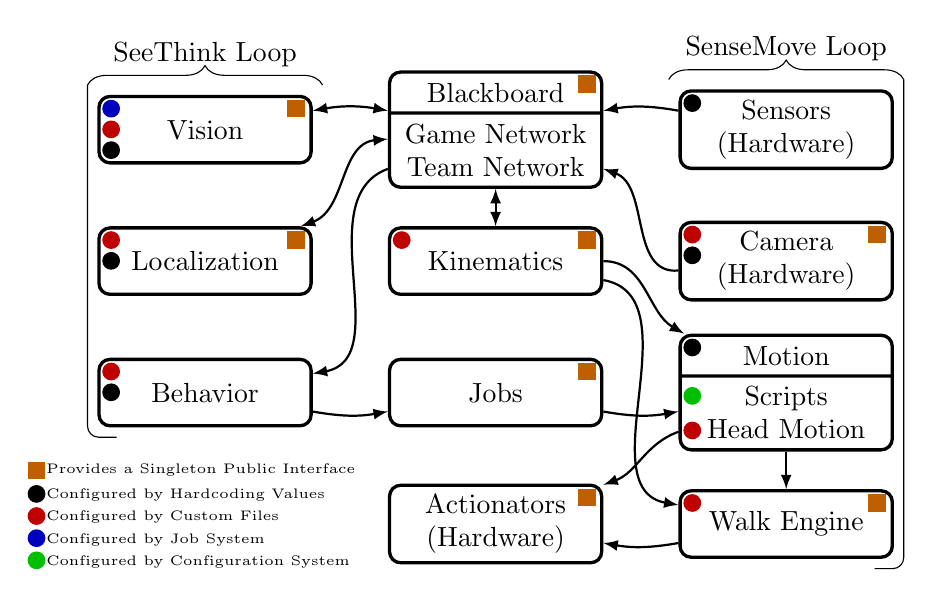
\begin{tikzpicture}[
            x=10.5em,y=4.75em,
            component/.style={
                rectangle
				, rounded corners
                , draw=black, very thick
                , text width=7em
                , minimum height=2.4em
                , text centered
            }
			, splitcomponent/.style={
				component
				, rectangle split
				, rectangle split parts=2
			}
			, configsystemconfig/.style={ color=green!75!black }
			, fileconfig/.style={ color=red!75!black }
			, jobconfig/.style={ color=blue!75!black }
			, hardcodedconfig/.style={ color=black }
			, publicinterface/.style={ color=orange!75!black}
            , write/.style={ ->, thick}
            , read/.style={<-, thick}
            , readwrite/.style={<->, thick}
            , >=latex
        ]

        %\node at (0.5,2.5) {$P_{1}$};

        %%% Nodes
        %% Left hand Side
        \node at (0,3) [component] (vision) {Vision};
        \node at (0,2) [component] (localization) {Localization};
        \node at (0,1) [component] (behavior) {Behavior};

        %% Center
        \node at (1, 3) [splitcomponent] (blackboard) {Blackboard \nodepart{two} Game Network\\Team Network};
		\node at (1, 2) [component] (kinematics) {Kinematics};
		\node at (1, 1) [component] (jobs) {Jobs};
		\node at (1, 0) [component] (actionators) {Actionators (Hardware)};

        %% Right hand side
        \node at(2,3) [component] (sensors) {Sensors (Hardware)};
        \node at(2,2) [component] (camera) {Camera (Hardware)};
        \node at(2,1) [splitcomponent] (motion) {Motion \nodepart{two} Scripts\\Head Motion};
        \node at(2,0) [component] (walkengine) {Walk Engine};

        %%% Connections
        %% Left side connections
        \path [readwrite, out=10, in=170] (vision) edge (blackboard);
        \path [readwrite, out=20, in=185] (localization) edge (blackboard);
        \path [read, out=10, in=200] (behavior) edge (blackboard);
		\path [write, out=-10, in=190] (behavior) edge (jobs);
		
		%% Center connections
        \path [readwrite] (kinematics) edge (blackboard);

        %% Right side connections
        \path [write, out=170, in=10] (sensors) edge (blackboard);
		\path [write, out=185, in=-20] (camera) edge (blackboard);
		\path [write, out=-10, in=190] (jobs) edge (motion);
		\path [write] (motion) edge (walkengine);
		\path [write, out=200, in=20] (motion) edge (actionators);
		\path [write, out=190, in=-10] (walkengine) edge (actionators);
		\path [read, out=150, in=0] (motion) edge (kinematics);
		\path [read, out=170, in=-10] (walkengine) edge (kinematics);
		
		%%% Configuration Colours
		%% Vision
		\filldraw[jobconfig] ([yshift=-.5em,xshift=.5em]vision.north west) circle(3pt);
		\filldraw[fileconfig] ([yshift=-1.25em,xshift=.5em]vision.north west) circle (3pt);
		\filldraw[hardcodedconfig] ([yshift=-2em,xshift=.5em]vision.north west) circle(3pt);
		\filldraw[publicinterface] ([yshift=-.8em,xshift=-0.9em]vision.north east) rectangle ++(6pt, 6pt);	
		
		%% Localization
		\filldraw[fileconfig] ([yshift=-.5em,xshift=.5em]localization.north west) circle(3pt);
		\filldraw[hardcodedconfig] ([yshift=-1.25em,xshift=.5em]localization.north west) circle (3pt);
		\filldraw[publicinterface] ([yshift=-.8em,xshift=-0.9em]localization.north east) rectangle ++(6pt, 6pt);
		
		%% Behavior
		\filldraw[fileconfig] ([yshift=-.5em,xshift=.5em]behavior.north west) circle(3pt);
		\filldraw[hardcodedconfig] ([yshift=-1.25em,xshift=.5em]behavior.north west) circle(3pt);
		
		%% Blackboard
		\filldraw[publicinterface] ([yshift=-.8em,xshift=-0.9em]blackboard.north east) rectangle ++(6pt, 6pt);
		
		%% Kinematics
		\filldraw[fileconfig] ([yshift=-.5em,xshift=.5em]kinematics.north west) circle(3pt);
		\filldraw[publicinterface] ([yshift=-.8em,xshift=-0.9em]kinematics.north east) rectangle ++(6pt, 6pt);
		
		%% Jobs
		\filldraw[publicinterface] ([yshift=-.8em,xshift=-0.9em]jobs.north east) rectangle ++(6pt, 6pt);
		
		%% Actionators
		\filldraw[publicinterface] ([yshift=-.8em,xshift=-0.9em]actionators.north east) rectangle ++(6pt, 6pt);
		
		%% Sensors
		\filldraw[hardcodedconfig] ([yshift=-.5em,xshift=.5em]sensors.north west) circle(3pt);
		
		%% Camera
		\filldraw[fileconfig] ([yshift=-.5em,xshift=.5em]camera.north west) circle(3pt);
		\filldraw[hardcodedconfig] ([yshift=-1.25em,xshift=.5em]camera.north west) circle (3pt);
		\filldraw[publicinterface] ([yshift=-.8em,xshift=-0.9em]camera.north east) rectangle ++(6pt, 6pt);
		
		%% Motion
		\filldraw[hardcodedconfig] ([yshift=-.5em,xshift=.5em]motion.north west) circle (3pt);
		\filldraw[configsystemconfig] ([yshift=-2.25em,xshift=.5em]motion.north west) circle (3pt);
		\filldraw[fileconfig] ([yshift=-3.5em,xshift=.5em]motion.north west) circle(3pt);
		
		%% Walk Engine
		\filldraw[fileconfig] ([yshift=-.5em,xshift=.5em]walkengine.north west) circle(3pt);
		\filldraw[publicinterface] ([yshift=-.8em,xshift=-0.9em]walkengine.north east) rectangle ++(6pt, 6pt);
		
		%%% Legend
		\coordinate (legendpoint) at (.55, .35);
		
		%% Public Interface
		\node [below=3pt of legendpoint,anchor=south east] (publicinterfacelabel) {\tiny Provides a Singleton Public Interface};
		\filldraw[publicinterface] ([yshift=-3pt,xshift=-3pt]publicinterfacelabel.west) rectangle ++(6pt, 6pt);

		%% Hard Coded Config
		\node [below=0.9em of publicinterfacelabel.south west,anchor=south west] (hardcodedconfiglabel) {\tiny Configured by Hardcoding Values};
		\filldraw[hardcodedconfig] ([yshift=.5pt]hardcodedconfiglabel.west) circle (3pt);
		
		%% File Config
		\node [below=0.8em of hardcodedconfiglabel.south west,anchor=south west] (fileconfiglabel) {\tiny Configured by Custom Files};
		\filldraw[fileconfig] ([yshift=.5pt]fileconfiglabel.west) circle (3pt);

		%% Job Config
		\node [below=0.8em of fileconfiglabel.south west,anchor=south west] (jobconfiglabel) {\tiny Configured by Job System};
		\filldraw[jobconfig] ([yshift=.5pt]jobconfiglabel.west) circle (3pt);

		%% Config System Config
		\node [below=0.8em of jobconfiglabel.south west,anchor=south west] (configsystemconfiglabel) {\tiny Configured by Configuration System};
		\filldraw[configsystemconfig] ([yshift=.5pt]configsystemconfiglabel.west) circle (3pt);
		
        %%% Decorations
        %% SeeThink header
        \node[fit=(vision)(localization)(behavior)](leftgroup){};
        \draw[rounded corners] 
        (leftgroup.north west)--(leftgroup.south west) -- ++(0.10,0);            
        \draw[decorate,decoration={amplitude=7pt,brace}] % Header line
        (leftgroup.north west) -- (leftgroup.north east);

        \node[above=1.1em of leftgroup,anchor=center]{SeeThink Loop};

        %% SenseMove header
        \node[fit=(sensors)(camera)(motion)(walkengine)](rightgroup){};
        \draw[rounded corners] 
        (rightgroup.north east) -- (rightgroup.south east) -- ++(-0.10,0);
        \draw[decorate,decoration={amplitude=7pt,brace}]
        (rightgroup.north west) -- (rightgroup.north east);
        \node[above=1.1em of rightgroup,anchor=center]{SenseMove Loop};
    \end{tikzpicture}

\end{frame}

\begin{frame}
    \frametitle{Existing Architecture}
    Description of Existing Architecture
\end{frame}

\subsection{Pain Points}
\begin{frame}
    \frametitle{Pain Points}
	Multiple ways to do the same thing
	Mix of different communication methods
	Threading
\end{frame}

%----------------------------------------------------------------------------------------
\section{NUClear Architecture}
%----------------------------------------------------------------------------------------
\subsection{Architectural Overview}
\begin{frame}[fragile]
    \frametitle{NUClear Architecure}
	\begin{adjustbox}{max totalsize={\textwidth}{.9\textheight},center}
	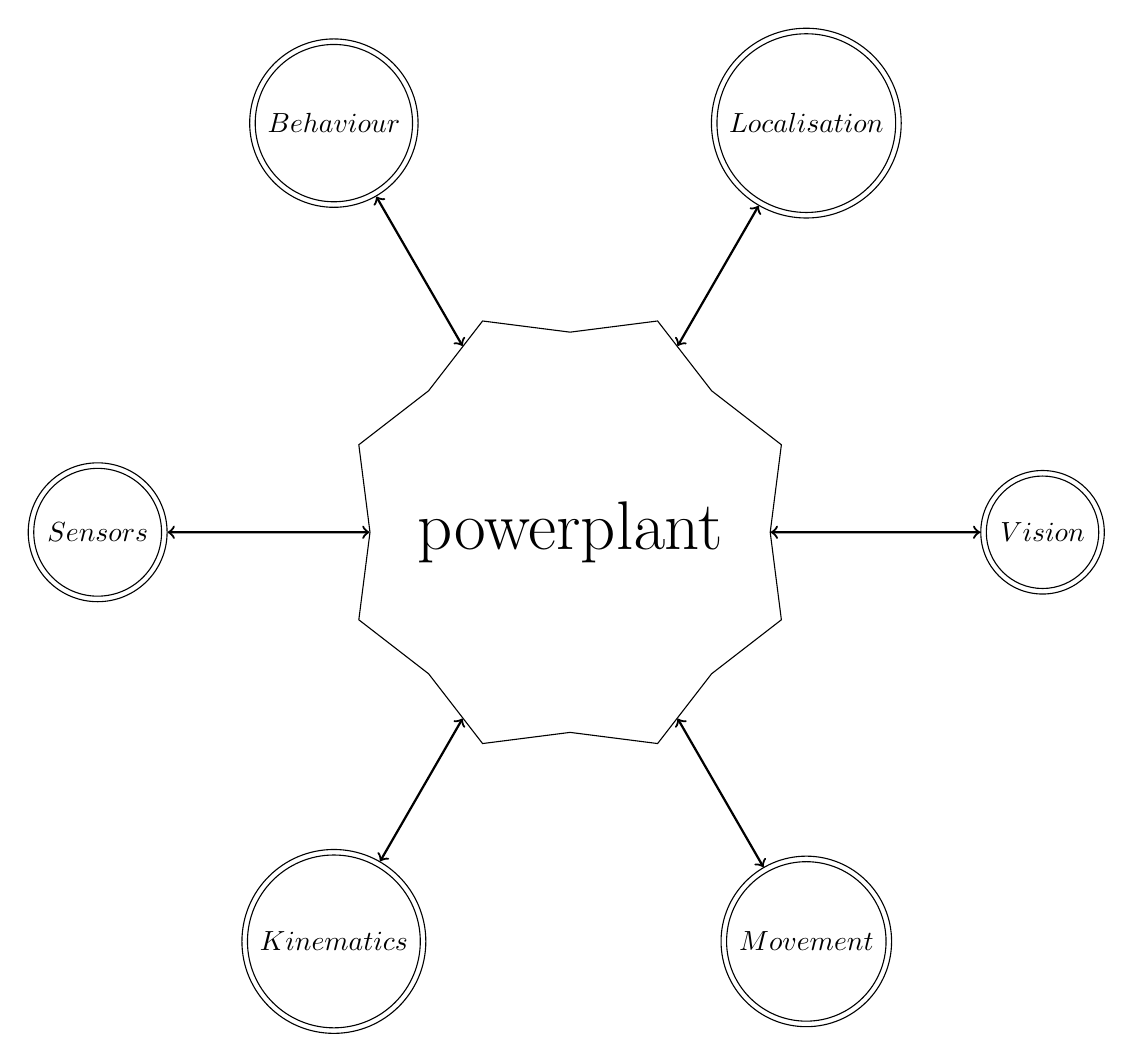
\begin{tikzpicture}[
		old inner xsep/.estore in=\oldinnerxsep,
		old inner ysep/.estore in=\oldinnerysep,
		double circle/.style 2 args={
			circle,
			old inner xsep=\pgfkeysvalueof{/pgf/inner xsep},
			old inner ysep=\pgfkeysvalueof{/pgf/inner ysep},
			/pgf/inner xsep=\oldinnerxsep+#1,
			/pgf/inner ysep=\oldinnerysep+#1,
			alias=sourcenode,
			append after command={
			let \p1 = (sourcenode.center),
			    \p2 = (sourcenode.east),
			    \n1 = {\x2-\x1-#1-0.5*\pgflinewidth}
			in
				node [inner sep=0pt, draw, circle, minimum width=2*\n1,at=(\p1),#2] {}
			}
		}
		, double circle/.default={2pt}{black}
		, reactor/.style={draw, double circle}
		, readwrite/.style={<->, thick}
	]
	
	% Draw our central Power Plant star
	\node [draw,star,star points=8,star point ratio=0.875,minimum width=5cm] (powerplant) {\Huge powerplant};
	
	% Loop through each of our reactors
	\foreach [count=\i] \reactor in {Vision,Localisation,Behaviour,Sensors,Kinematics,Movement} {
	
		% Draw the reactors around the central star
		\node[draw,reactor] (reactorcircle) at ({360/6 * (\i - 1)}:6cm) {$\reactor$};
	
		% Draw a line from our reactor to our powerplant
		\path[readwrite] (reactorcircle) edge (powerplant);
	};
	\end{tikzpicture}
	\end{adjustbox}

\end{frame}

\begin{frame}
    \frametitle{NUClear Architecure}
	Message passing system,
	Multi Threading,
	Networking,
	Power Plant,
	Reactors,
	Reactions
	Smart Types
	Extensions
	Service Threads
\end{frame}

\begin{frame}
	High Level On Description
\end{frame}

\begin{frame}
	Trigger
\end{frame}

\begin{frame}
	With
\end{frame}

\begin{frame}
	Options
\end{frame}

\subsection{Key Functions}
\begin{frame}[fragile]
    \frametitle{Key Functions: On}
	\begin{lstlisting}[language=nuclear]
	// Vision.cpp
	Vision::Vision() {
	    using messages::Image;
	    on<Trigger<Image>>([this](const Image& image) {
	        auto classifedImage = classifyImage(image);
	        emit(std::move(classifiedImage));
	    });
	}
	\end{lstlisting}
\end{frame}

\begin{frame}
    \frametitle{Key Functions Emit}
	Default
	Scopes
	Unique Pointers
	Code Example
\end{frame}

\begin{frame}
    \frametitle{Key Functions Log}
	Stream operator overload
	variardic
\end{frame}

\begin{frame}
    \frametitle{Key Functions Log}
	Every
\end{frame}

\begin{frame}
    \frametitle{Key Functions Log}
	Last
\end{frame}

\begin{frame}
    \frametitle{Key Functions Log}
	Configuration
\end{frame}


\begin{frame}
    \frametitle{Key Functions Log}
	Project Directory Structure
\end{frame}

\begin{frame}
    \frametitle{Antipatterns}
	unending loops in reactions
\end{frame}

\subsection{Module Examples}
\begin{frame}
    \frametitle{Some title}
	Config System
	Party Darwin
	Show examples
\end{frame}

\subsection{Current Porting Status}
\begin{frame}
    \frametitle{Current Porting Status}
	What has been ported
\end{frame}

\end{document} 
